\chapter{Evaluation and Testing}
It is important to test the system. Not only manually testing the website, but also empirically testing the efficient of the recommender system. One of the main problems that we have is that we do not have an original dataset to test our system, we discuss ways of overcoming this issue in section \ref{coldStartProble}.
\section{Quality of Recommender systems}
\subsection{Evaluation Metrics}
The quality of recommender systems can evaluated using a variety of different empirical metrics \cite{isinkaye2015recommendation}. We use empirical methods because it gives us a statistical value we can aim to improve. It also gives us a value we can compare against other recommender systems, allowing us to measure against industry standards and benchmarks
\subsection{Extreme Cold Start Problem} \label{coldStartProble}
To test our machine learning model, we would need to have training data to train our model on and then calculate the MSE to know how accurate our model is. However, as this is a completely new system, there is no previous data-set to train the machine learning model on which means that there is no way to test the model. One of the way's to solve this problem is to generate our own dataset.

\subsubsection{Generating Dataset}
Although this will not be an accurate dataset to train our model on, it would help test how good the machine learning model we created is. For the dataset we to need to generate users and routes. For each user and route, we assign 4 attributes: Terrain, Distance, Elevation and Scenery (representing four attributes of a route). For each user, we generate values for these attributes that will correspond with how much each user likes that attribute for a route as shown in table \ref{tab:genUserDataset}. 

The attribute values range from 0 to 9, 0 g extreme dislike and 9 meaning extreme like. Each route will also have values for this attributes which is how much of that attribute that the route has as shown in table \ref{tab:genRouteDataset}.

\begin{table}[ht]
    \centering
    \begin{tabular}{|c|c|c|c|c|}
        \hline
         User ID & Terrain & Distance & Elevation & Scenery  \\
         \hline
         \hline
         0 & 3 & 1 & 3 & 7  \\
         1 & 7 & 8 & 1 & 2 \\
         2 & 8 & 0 & 5 & 2 \\
         4 & 6 & 7 & 7 & 2 \\
         \hline
    \end{tabular}
    \caption{Example of User Data to help generate dataset}
    \label{tab:genUserDataset}
\end{table}

\begin{table}[ht]
    \centering
    \begin{tabular}{|c|c|c|c|c|}
        \hline
         Route ID & Terrain & Distance & Elevation & Scenery  \\
         \hline
         \hline
         0 & 5 & 1 & 3 & 7  \\
         1 & 7 & 5 & 1 & 2 \\
         2 & 8 & 0 & 5 & 8 \\
         4 & 6 & 7 & 7 & 9 \\
         \hline
    \end{tabular}
    \caption{Example of Route Data to help generate dataset}
    \label{tab:genRouteDataset}
\end{table}

We generate 30 users with 5 each from the sub classes in table \ref{tab:attributeSubClasses}. The sub classes are an attempt to represent different types of users and the attribute values are to reflect what they look for int trails. We also generate 60 routes with 10 from each of the sub classes in table \ref{tab:attributeSubClasses}.
\begin{table}[ht]
    \centering
    \begin{tabular}{|c|c|c|c|c|}
        \hline
         Sub-classes & Terrain & Distance & Elevation & Scenery \\
         \hline
         Hardcore & 7 - 9 & 7 - 9 & 7 - 9 & 0 - 9 \\  
         \hline
         Distance & 0 - 3 & 7 - 9 & 0 - 3 & 0 - 3 \\
         \hline
         Visual & 0 - 3 & 0 - 3 & 0 - 3 & 7 - 9 \\
         \hline
         Mountain & 0 - 3 & 0 - 3 & 7 - 9 & 0 - 3 \\
         \hline
         Casual & 0 - 3 & 0 - 3 & 0 - 3 & 0 - 3 \\
         \hline
         Random & 0 - 9 & 0 - 9 & 0 - 9 & 0 - 9 \\
         \hline
    \end{tabular}
    \caption{Caption}
    \label{tab:attributeSubClasses}
\end{table}

Each user runs and rates between 10 and 23 random routes from the generated routes. For each user and the route they run we calculate a \textit{like} value using the attribute values from the user and the route using equation \ref{eqn:Likes}. We then add another probability value that is created using a Gaussian Probability Distribution\cite{simon2007probability} to create and equal probability distribution. This probability value is to add a little bit of randomness to the like value. This represents if for example it was raining when a user runs a route which can affect how they feel about the route compared to normal conditions.

We then use this like value to calculate the rating by using the equation \ref{eqn:RatingCalculation}. We use the Sigmoid function\cite{wiki:SigmoidFunction}, which is a non-linear function\footnote{It's normally used as an activation function in neural networks}, that can map the calculated like value to a value between 0 - 1.

\begin{equation} \label{eqn:Likes}
    \textrm{likes} = \Bigg(\sum_{i=1}^{n=4}abs({u_i}-{r_i})\Bigg) + {p_i}
\end{equation}

\begin{equation} \label{eqn:RatingCalculation}
    \textrm{rating} = \big(\sigma(\textrm{likes}) \times 4\big) + 1
\end{equation}

We then use these generated ratings to help train our machine learning model. With tensor flow we can get our final MSE and root it to get our Root Mean Squared Error (RMSE), the standard for comparing how good the recommender system machine learning models are.

\subsection{Movie Lens Data-set}
Another way to test the system is to use an already existing dataset. One of the benefits of recommender systems is that it can be applied to any generic user-item ratings matrix. Hence although we may not be able to find an already existing user-route ratings matrix, we can use another user-item ratings matrix to test it.

The dataset that I used is a popular dataset of user-movies ratings called the Movie lens Dataset\footnote{https://grouplens.org/datasets/movielens/}. The best thing about using this data set is that there are other online recommender systems that have been tested on this dataset that we can compare our RMSE score against\footnote{https://www.kaggle.com/learn/overview}\footnote{https://www.librec.net/release/v1.3/example.html}.

Create another model that is trained on our movie lens dataset based on the exact same code as the one for our original neural network model.

\section{Manual Testing}
\subsection{GraphQL Dev Tools}
\begin{figure}[ht]
    \centering
    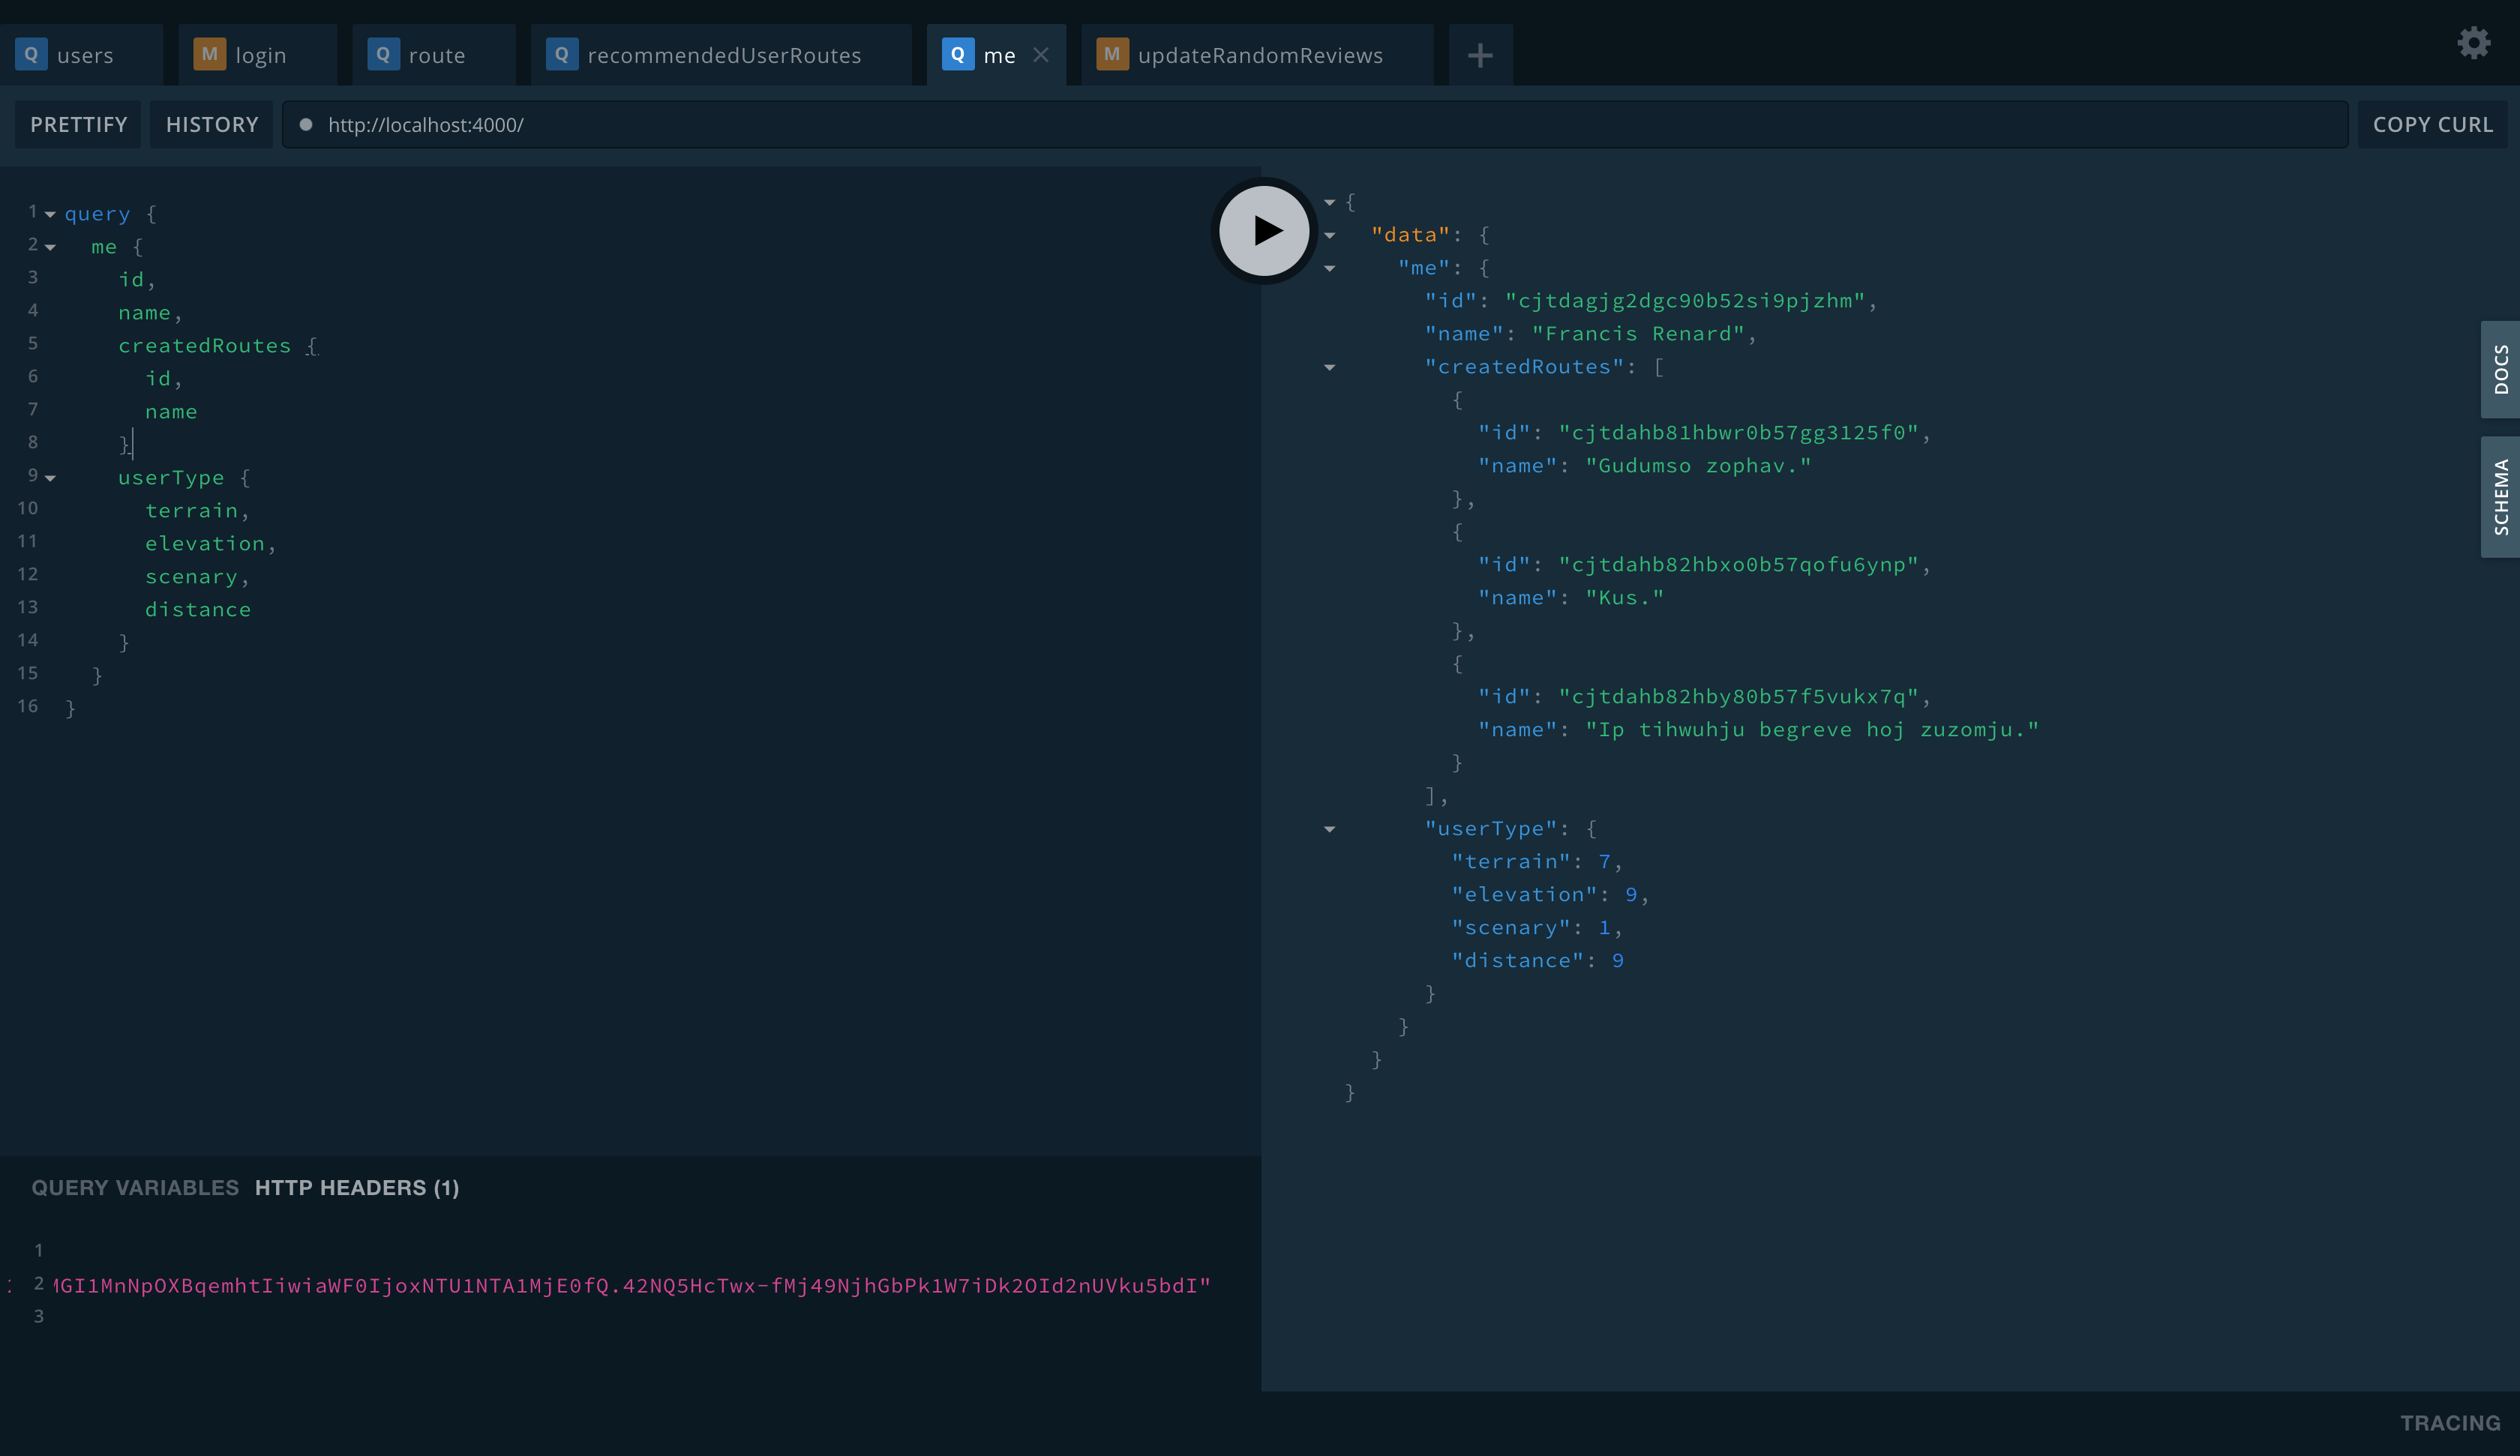
\includegraphics[width=\textwidth]{graphql-dev.png}
    \caption{GraphQl Development Tools}
    \label{fig:graphQLDevTools}
\end{figure}

\subsection{Redux Dev Tools}
NgRx comes with dev tools as shown in figure \ref{fig:reduxDevTools}. It allows us to track the state of our application as it evolves from initial login, to router navigations and trail changes. This record can then be used to rewind through previous actions, allowing us to provide undo and redo functionalities to the user.
\begin{figure}[ht]
    \centering
    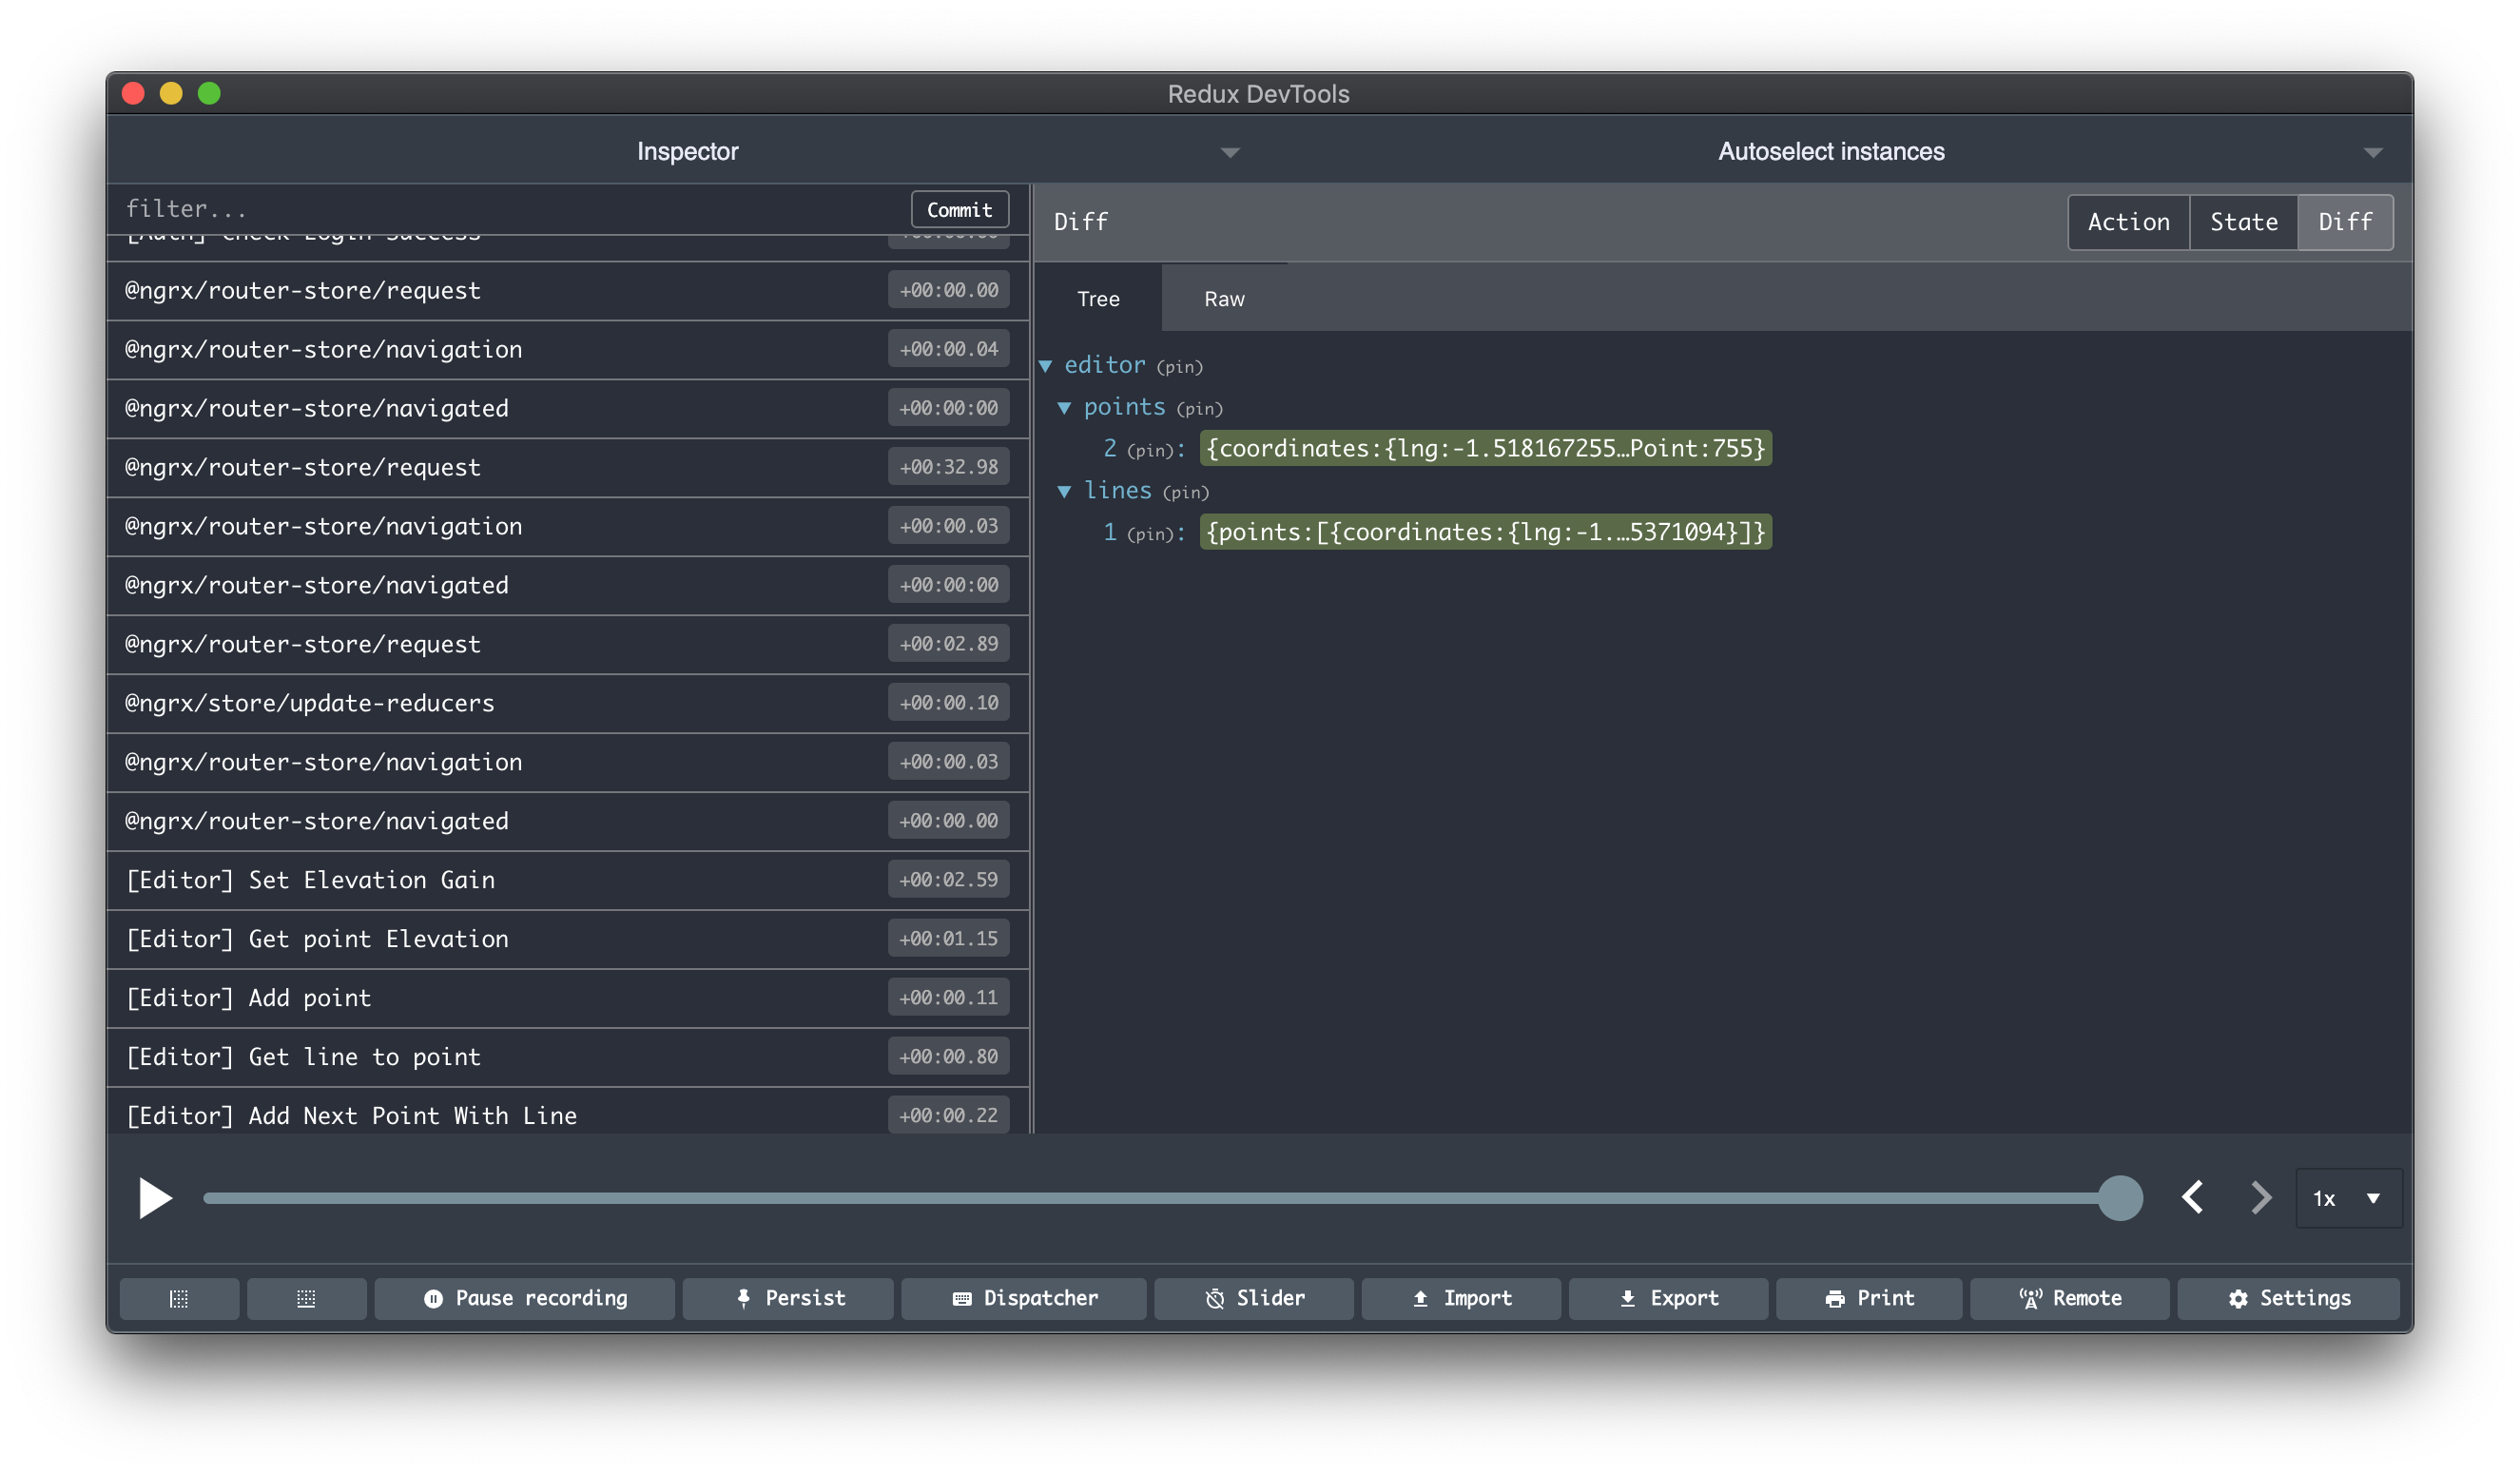
\includegraphics[width=\textwidth]{redux-dev-tools.png}
    \caption{Redux Dev Tools}
    \label{fig:reduxDevTools}
\end{figure}


\section{Unit and Integration Testing}
To test the frontend we follow a standard industry methods of creating both unit tests and integration tests. Angular comes built with the Jasmine Testing framework\footnote{https://jasmine.github.io/}, a javascript behaviour driven framework. Jasmine also use Karma\footnote{https://karma-runner.github.io/latest/index.html}, that allows us to run the tests on the browser.

Angular also provides Protractor\footnote{https://www.protractortest.org/} for end to end testing on the front end